%!TEX root = A0.Master.tex
\chapterbegin{Descripción de la aplicación: cliente y servidor}

La aplicación desarrollada en el presente proyecto está compuesta por dos partes fundamentales: el proveedor de datos situado en un servidor remoto, y la aplicación del dispositivo móvil, que pide datos al servidor e interpreta en la pantalla del usuario dichos resultados.

Como ya se ha comentado en el primer capítulo, la parte del servidor no será descrita por completo ya que no entra dentro del ámbito de este Proyecto de Fin de Carrera.

\section{Cliente}
En esta sección nos concentraremos en describir la aplicación cliente que el usuario dispondrá en su iPhone. Este cliente debe proporcionar de manera rápida y eficaz la información que necesita el usuario. Para ello se ha diseñado un sistema de navegación de varios pasos consecutivos, simplificando la UI al máximo para cumplir los requisitos de rapidez y eficacia, teniendo en mente siempre que el usuario utilizará nuestra aplicaciones por un tiempo menor de 30 segundos, ya que se encuentra ocupado comprando en la tienda física. En la Figura \ref{fig:esqueleto} se muestra el esqueleto de nuestra aplicación cliente.

\begin{figure}[H]
	\centering
		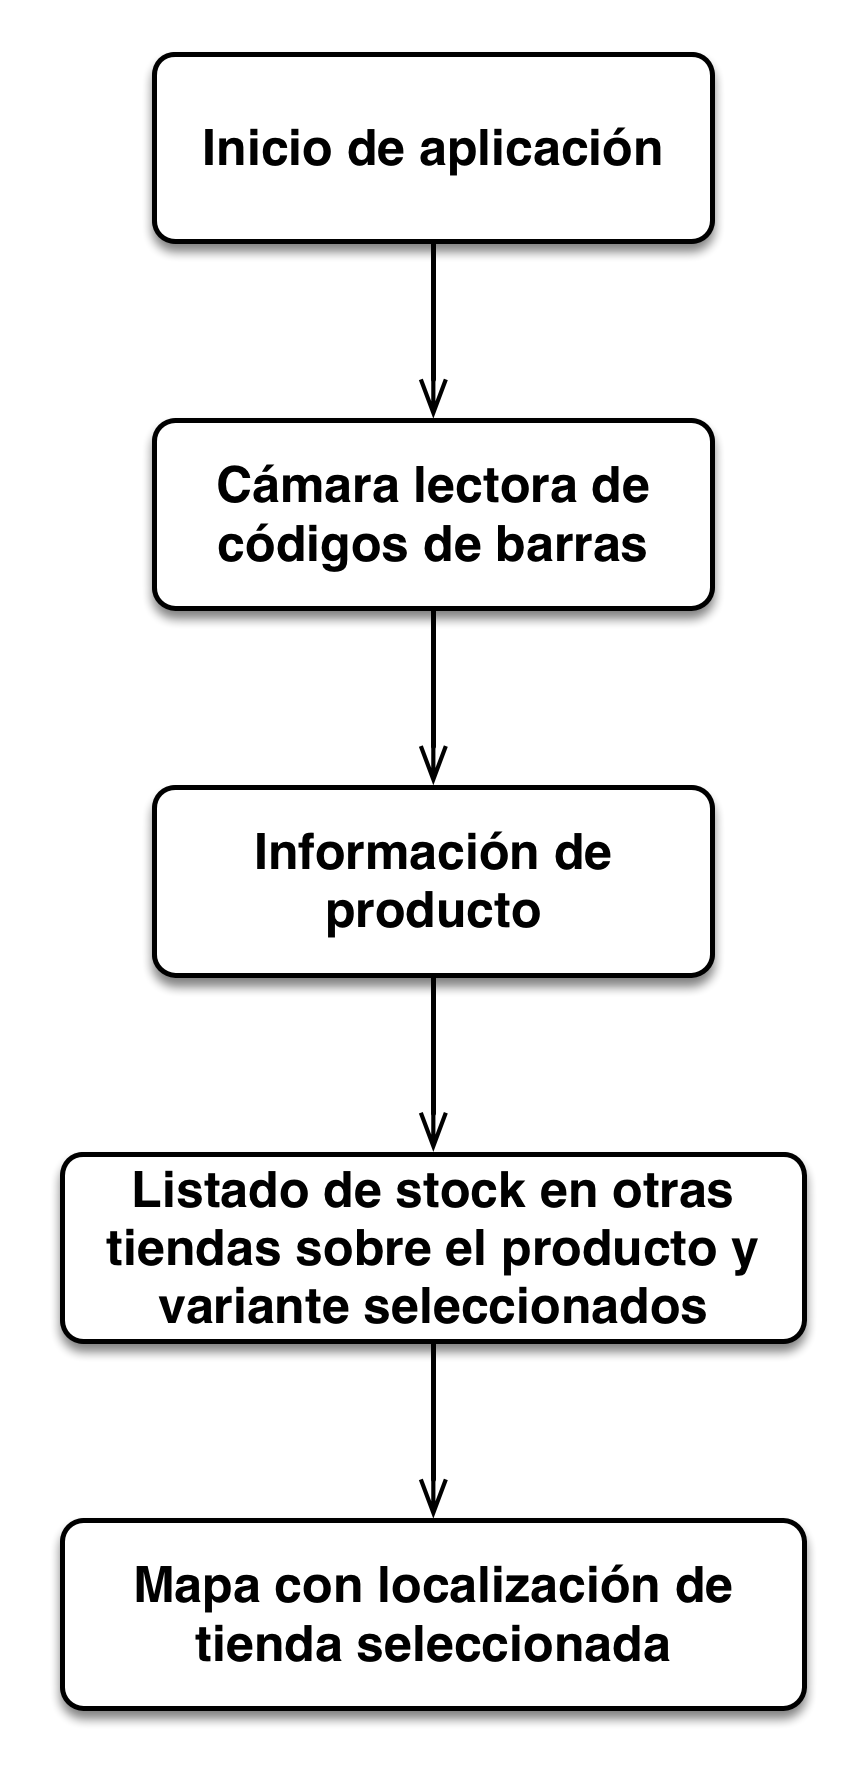
\includegraphics[width=0.4\textwidth]{./img/esqueleto-app.png}
	\caption{Esqueleto de navegación entre pantallas de la aplicación móvil cliente del usuario.}
	\label{fig:esqueleto}
\end{figure}

\subsection{Pantallas del cliente}
La aplicación móvil dispone de una pantalla de inicio, una pantalla que previsualiza la imagen capturada por la cámara trasera del móvil, una pantalla que muestra el producto escaneado, una pantalla que lista las diferentes tiendas con el stock actual de dicho producto, y una mapa que muestra la posición actual del usuario y de la tienda seleccionada en la pantalla anterior.

\begin{figure}[H]
	\centering
		\frame{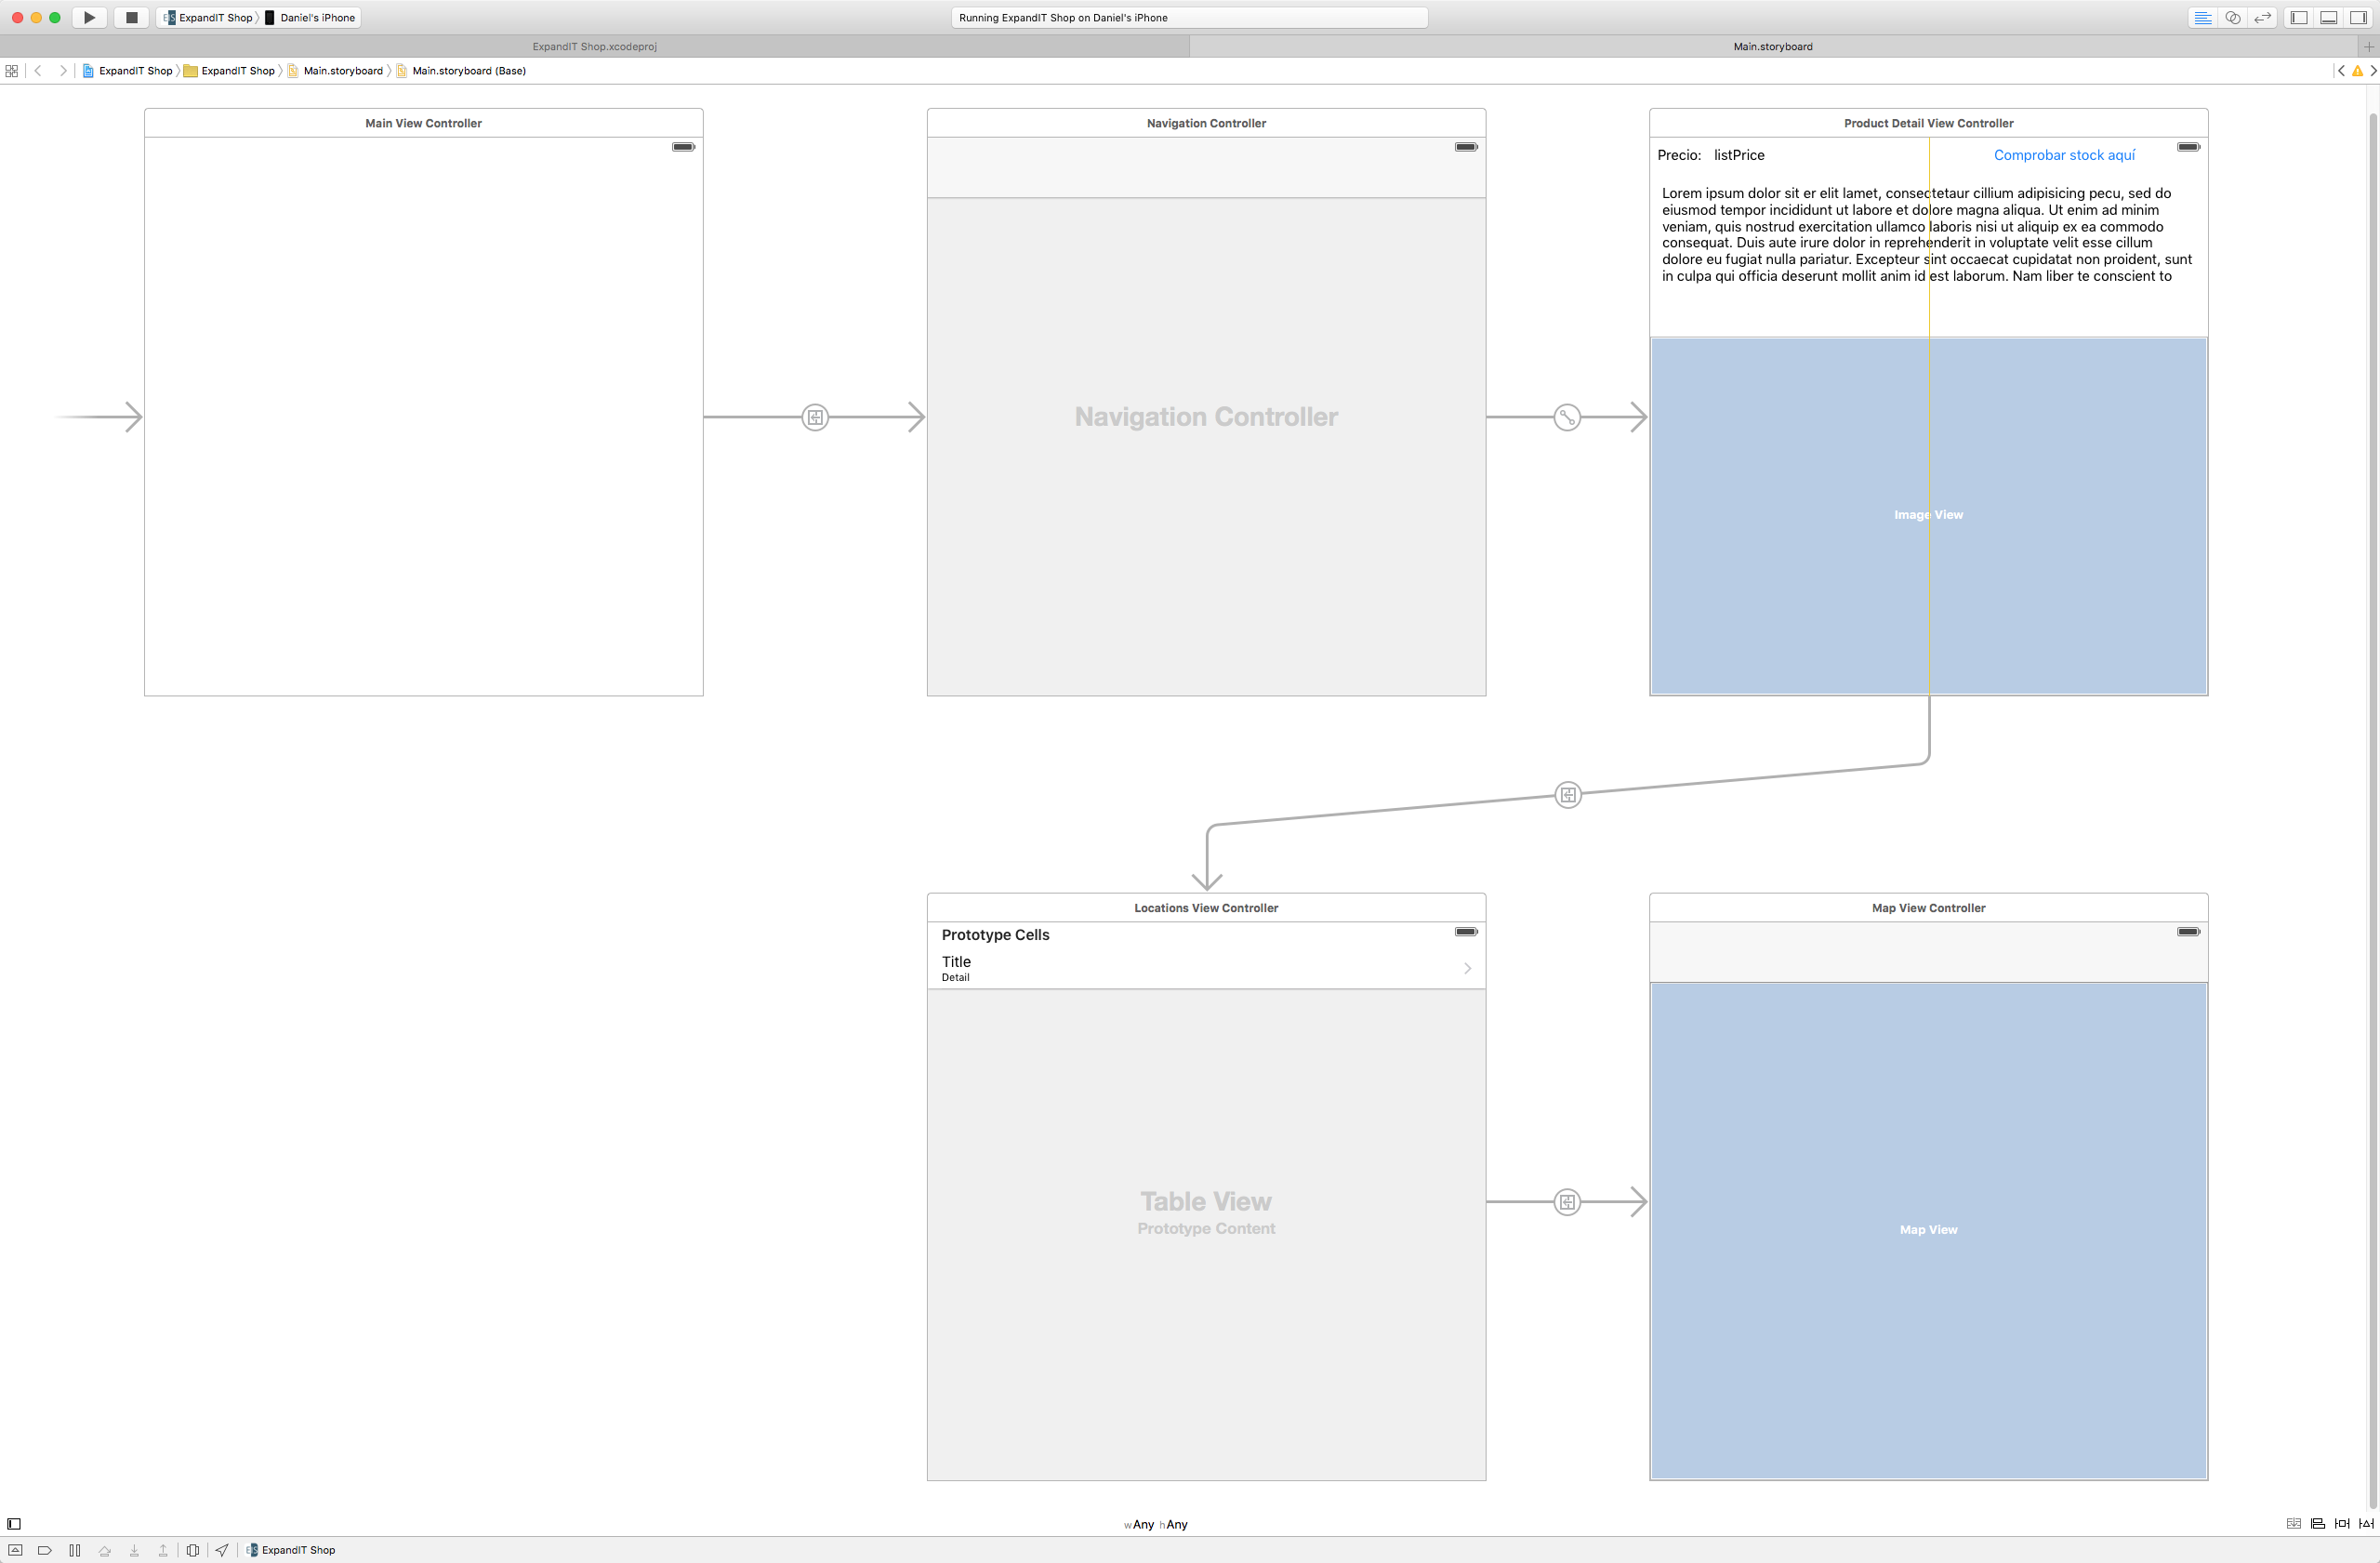
\includegraphics[width=1\textwidth]{./img/storyboard.png}}
	\caption{Previsualización en \emph{Storyboard} de las pantallas de la aplicación cliente.}
	\label{fig:storyboard}
\end{figure}

A continuación se describirá cada una de las pantallas que componen nuestra aplicación. El dispositivo utilizado para el desarrollo es un iPhone 5 con una resolución de 1136x640 píxeles, aunque esto no supone ningún impedimento para mostrar la aplicación en otras resoluciones gracias al uso de AutoLayout.

Esta tecnología permite definir las reglas por las que se rigen los elementos en pantalla (campos de texto, botones, etc.) en vez de definir unas medidas exactas.

\subsubsection{Pantalla de inicio}
La aplicación móvil dispone de una pantalla de inicio que muestra el logotipo de la empresa que ha encargado la creación de la app. Este proceso es requerido por Apple si se desea publicar la aplicación en la App Store. El tiempo que esta pantalla es mostrada dependerá de la velocidad con la que se inicia la aplicación.

%% TO DO: Poner imagen de la UMA y hacer captura.

\subsubsection{Pantalla de inicio: cámara}
Lo primero que verá el usuario en pantalla será la propia imagen de la cámara, lista para capturar un código de barras. El decodificador de barras está programado de manera que únicamente reconozca el formato \emph{Code 128}. En caso de lectura de un código que no pertenezca a ningún producto, se muestra un mensaje de error.

\begin{figure}[H]
	\centering
		\frame{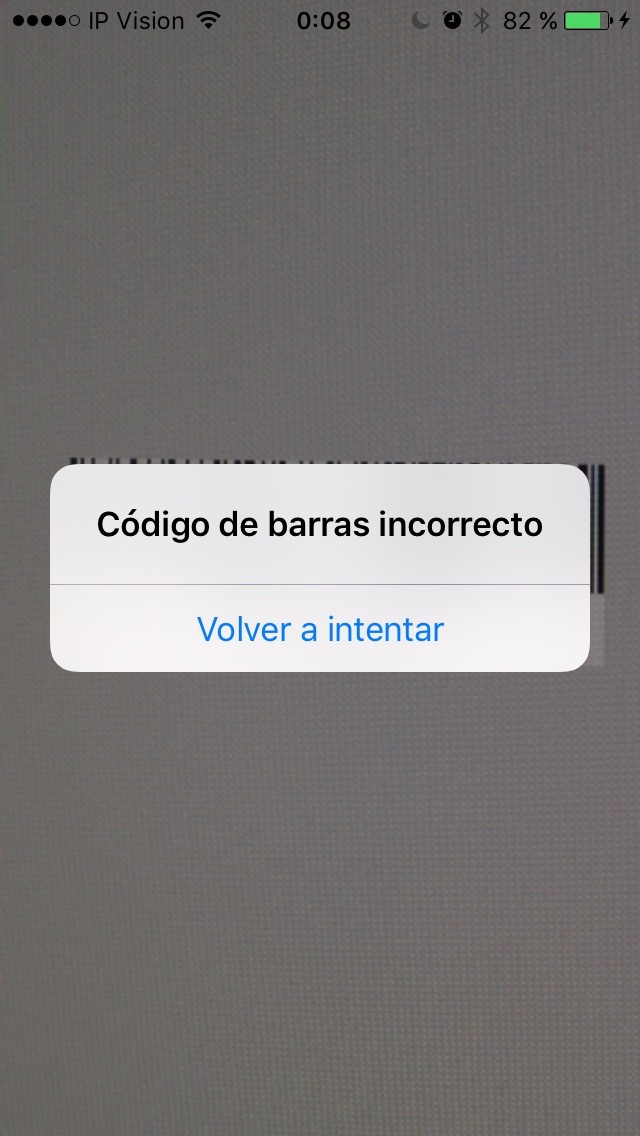
\includegraphics[width=0.5\textwidth]{./img/screenshot-camara-error.jpg}}
	\caption{Mensaje de error mostrado al usuario cuando el código de barras es incorrecto.}
	\label{fig:codigoBarrasError}
\end{figure}

\subsubsection{Pantalla de información de producto} \label{sssec:pantalla-info-producto}
Una vez que se ha escaneado un código de barras válido, el servidor buscará en su base de datos el producto y devolverá el resultado en JSON. La aplicación cliente es la encargada de parsear el mensaje y mostrar en pantalla el nombre del producto, precio, descripción y una imagen.

\begin{figure}[H]
	\centering
		\frame{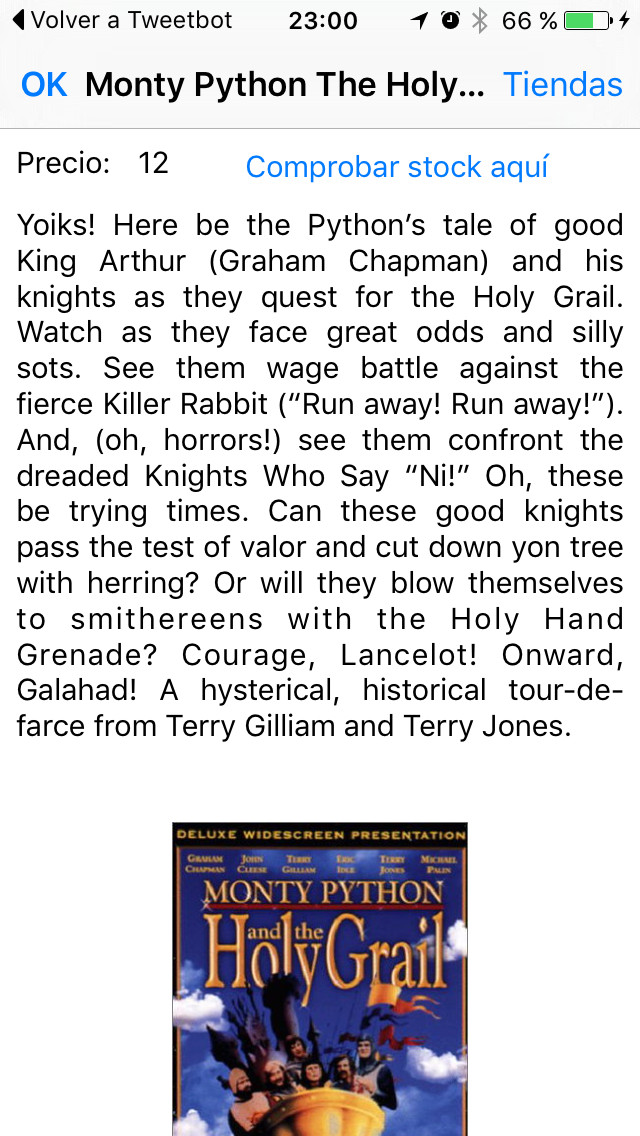
\includegraphics[width=0.5\textwidth]{./img/screenshot-info-producto.png}}
	\caption{Pantalla de información del producto escaneado. Muestra el nombre del producto, el precio, una descripción, una imagen y un botón para pedir el número de productos en stock.}
	\label{fig:infoProducto}
\end{figure}

También se muestra un botón con el cual el usuario verificará el stock de dicho producto en la posición actual del dispositivo.

Cuando el usuario presiona este botón, se envía al servidor una petición cuyos parámetros son el código de producto, la latitud y longitud del dispositivo, y la precisión con la que el GPS ha operado.

\begin{figure}[H]
	\centering
		\frame{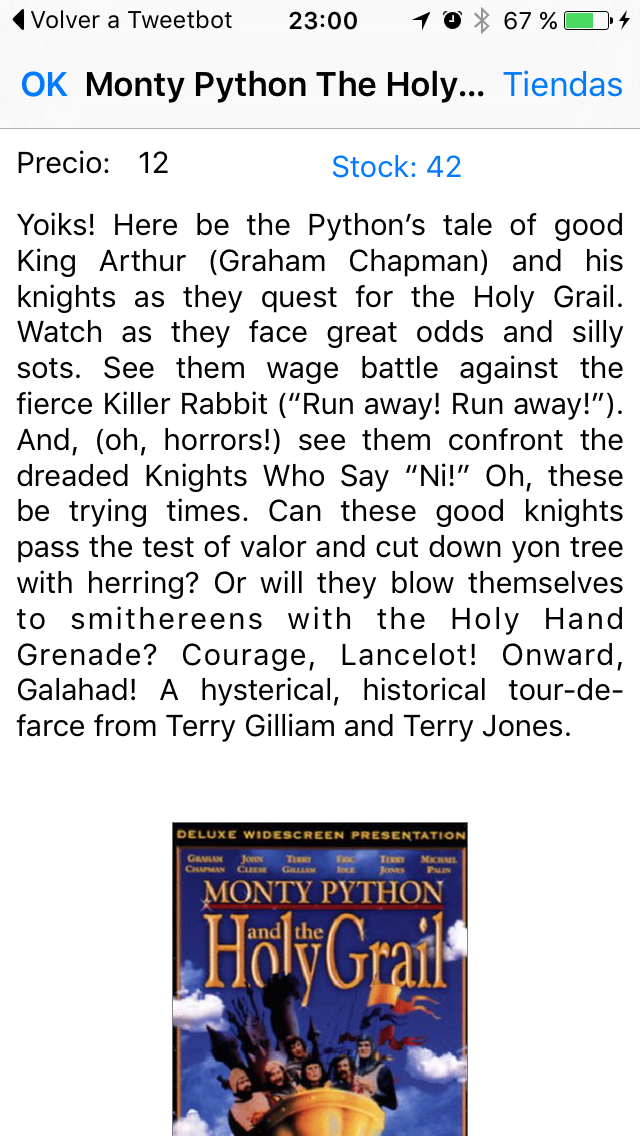
\includegraphics[width=0.5\textwidth]{./img/screenshot-boton-stock.png}}
	\caption{Cuando se presiona el botón de comprobación de stock, este cambia el texto del botón por el stock del producto.}
	\label{fig:botonStock}
\end{figure}

Si el cálculo de la posición del usuario con respecto a la tienda más cercana diera como resultado que no se encuentra en alguno de los comercios que están almacenados en la base de datos o la precisión del GPS no es suficiente, se procede a mostrar un mensaje de error.

\begin{figure}[H]
	\centering
		\frame{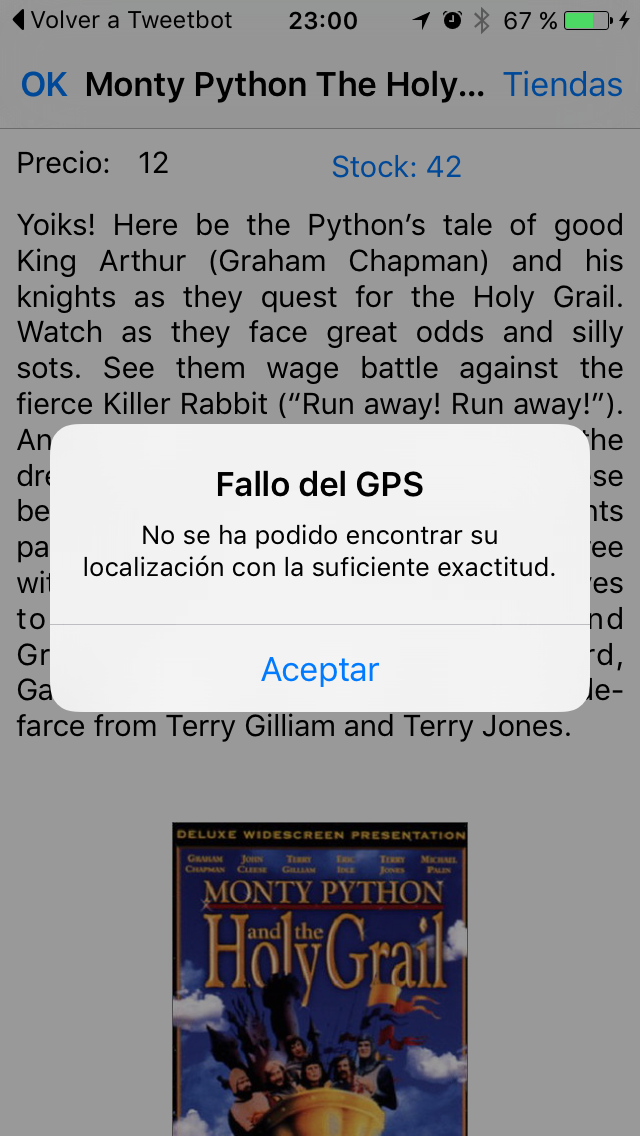
\includegraphics[width=0.5\textwidth]{./img/screenshot-error-gps.png}}
	\caption{Mensaje de error al no localizar al usuario dentro de una tienda.}
	\label{fig:errorGPS}
\end{figure}

\subsubsection{Pantalla de lista de tiendas con stock}
Al pulsar sobre el botón ``Tiendas'', el servidor nos devuelve un mensaje con un array en JSON. Cada elemento del array supone un objeto con información de cada tienda y del stock del producto seleccionado en cada una de ellas. Este array es transformado para ser mostrado en una \texttt{UITableView}.

\begin{figure}[H]
	\centering
		\frame{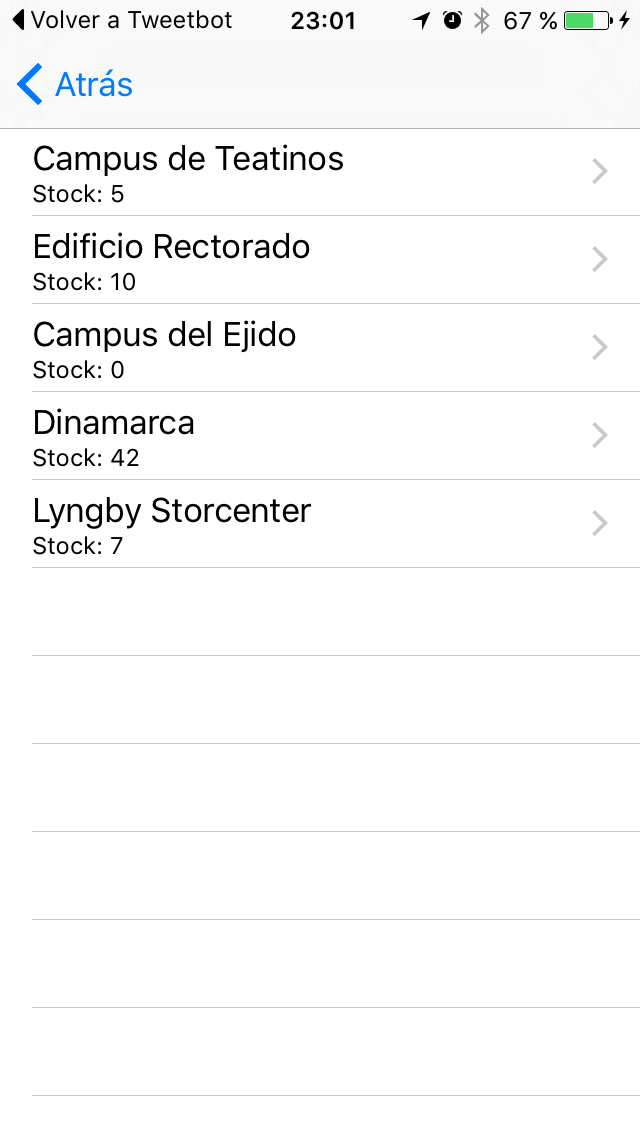
\includegraphics[width=0.5\textwidth]{./img/screenshot-lista-tiendas.png}}
	\caption{Listado de tiendas que muestra el stock del producto en cada una de ellas.}
	\label{fig:listaTiendas}
\end{figure}

\subsubsection{Pantalla de mapa con tienda geolocalizada}
La última pantalla a la que puede llegar el usuario muestra un mapa con la localización del usuario y de la tienda seleccionada.

\begin{figure}[H]
	\centering
		\frame{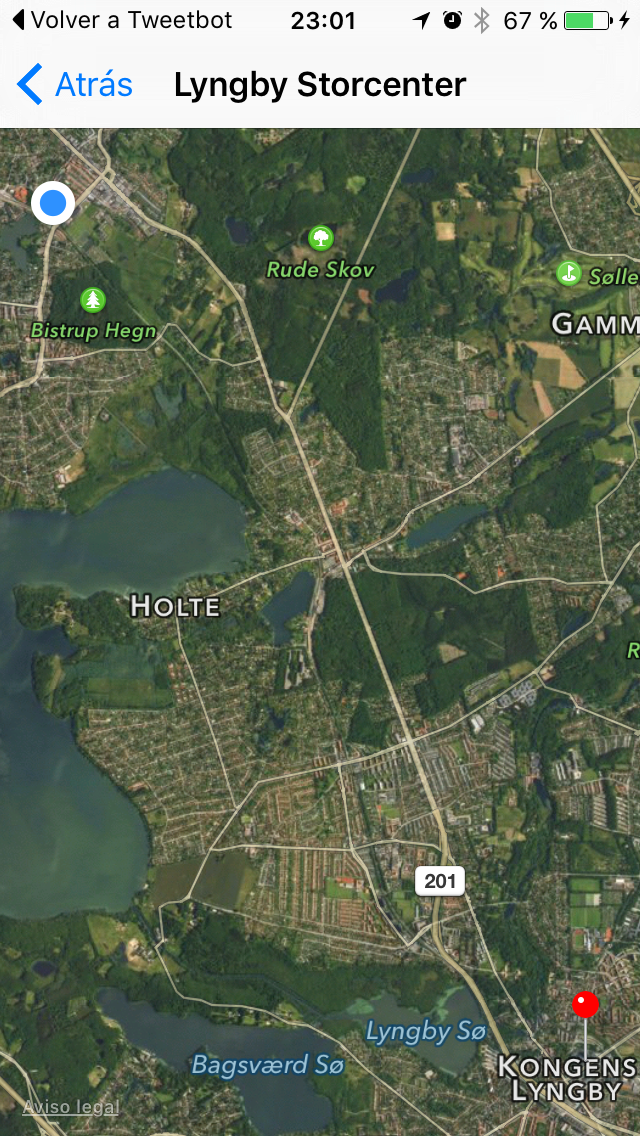
\includegraphics[width=0.5\textwidth]{./img/screenshot-mapa1.png}}
	\caption{En el mapa se muestra la ubicación del usuario (punto azul) y de la tienda seleccionada (chincheta roja).}
	\label{fig:mapa}
\end{figure}

Cuando el usuario presiona sobre el marcador rojo de la tienda, una anotación aparece y permite al usuario visitar la página web asociada a dicho comercio (si está especificada en la base de datos).

\begin{figure}[H]
	\centering
		\frame{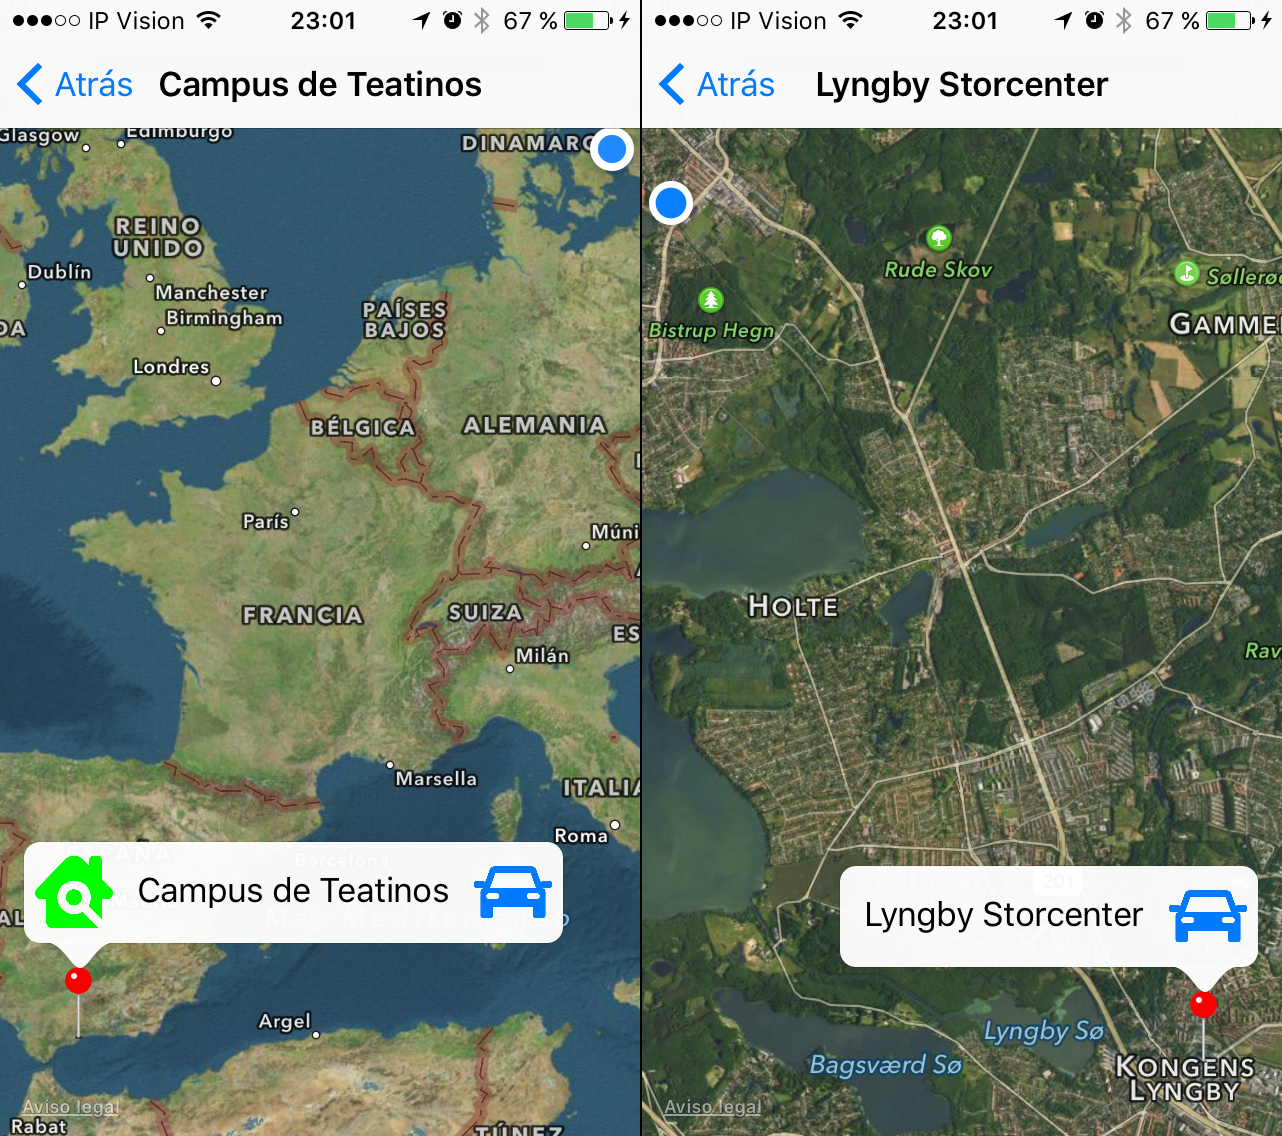
\includegraphics[width=0.8\textwidth]{./img/screenshot-mapa-anotaciones.png}}
	\caption{Las anotaciones de tiendas pueden llevar un icono que redirige a su página web (izquierda) o carecer de ello (derecha).}
	\label{fig:mapa-anotaciones}
\end{figure}

El usuario también puede ordenar a la aplicación iniciar una ruta con navegación paso por paso desde la ubicación actual hasta la tienda destino, tal y como se muestra en la Figura \ref{fig:mapa-ruta}.

\begin{figure}[H]
	\centering
		\frame{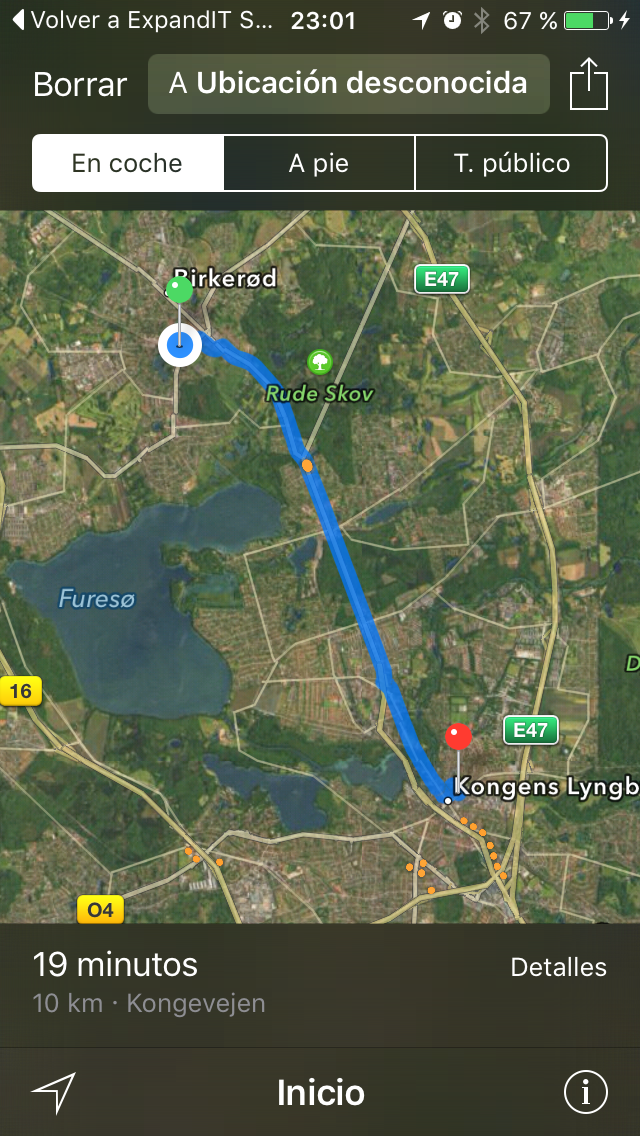
\includegraphics[width=0.5\textwidth]{./img/screenshot-ruta.png}}
	\caption{La aplicación envía al usuario a la app Maps para iniciar una navegación paso por paso.}
	\label{fig:mapa-ruta}
\end{figure}

\subsection{Petición y recepción de datos del servidor en el cliente}
Como ya se ha comentado anteriormente, la aplicación cliente realiza peticiones al servidor, que devuelve los datos en formato JSON. Dependiendo de la pantalla en la que se encuentre el usuario, la aplicación realizará una llamada u otra.

En la Figura \ref{fig:diagrama-camara} se muestra la secuencia de comunicación entre cliente y servidor que se produce en la lectura de un código de barras y búsqueda del producto correspondiente. En primer lugar, en el cliente se inicia la cámara (primeramente se debe pedir permiso al usuario para usar la cámara) y comienza el proceso de lectura constante en busca de un código de barras válido (en nuestro caso \emph{Code 128}). Tras la lectura de un código de barras válido, el cliente envía una llamada al servidor con la función \texttt{getProduct:} y el identificador decodificado del código de barras. El servidor devuelve un documento JSON con la información del producto seleccionado o un código de error.

\begin{figure}[H]
	\centering
		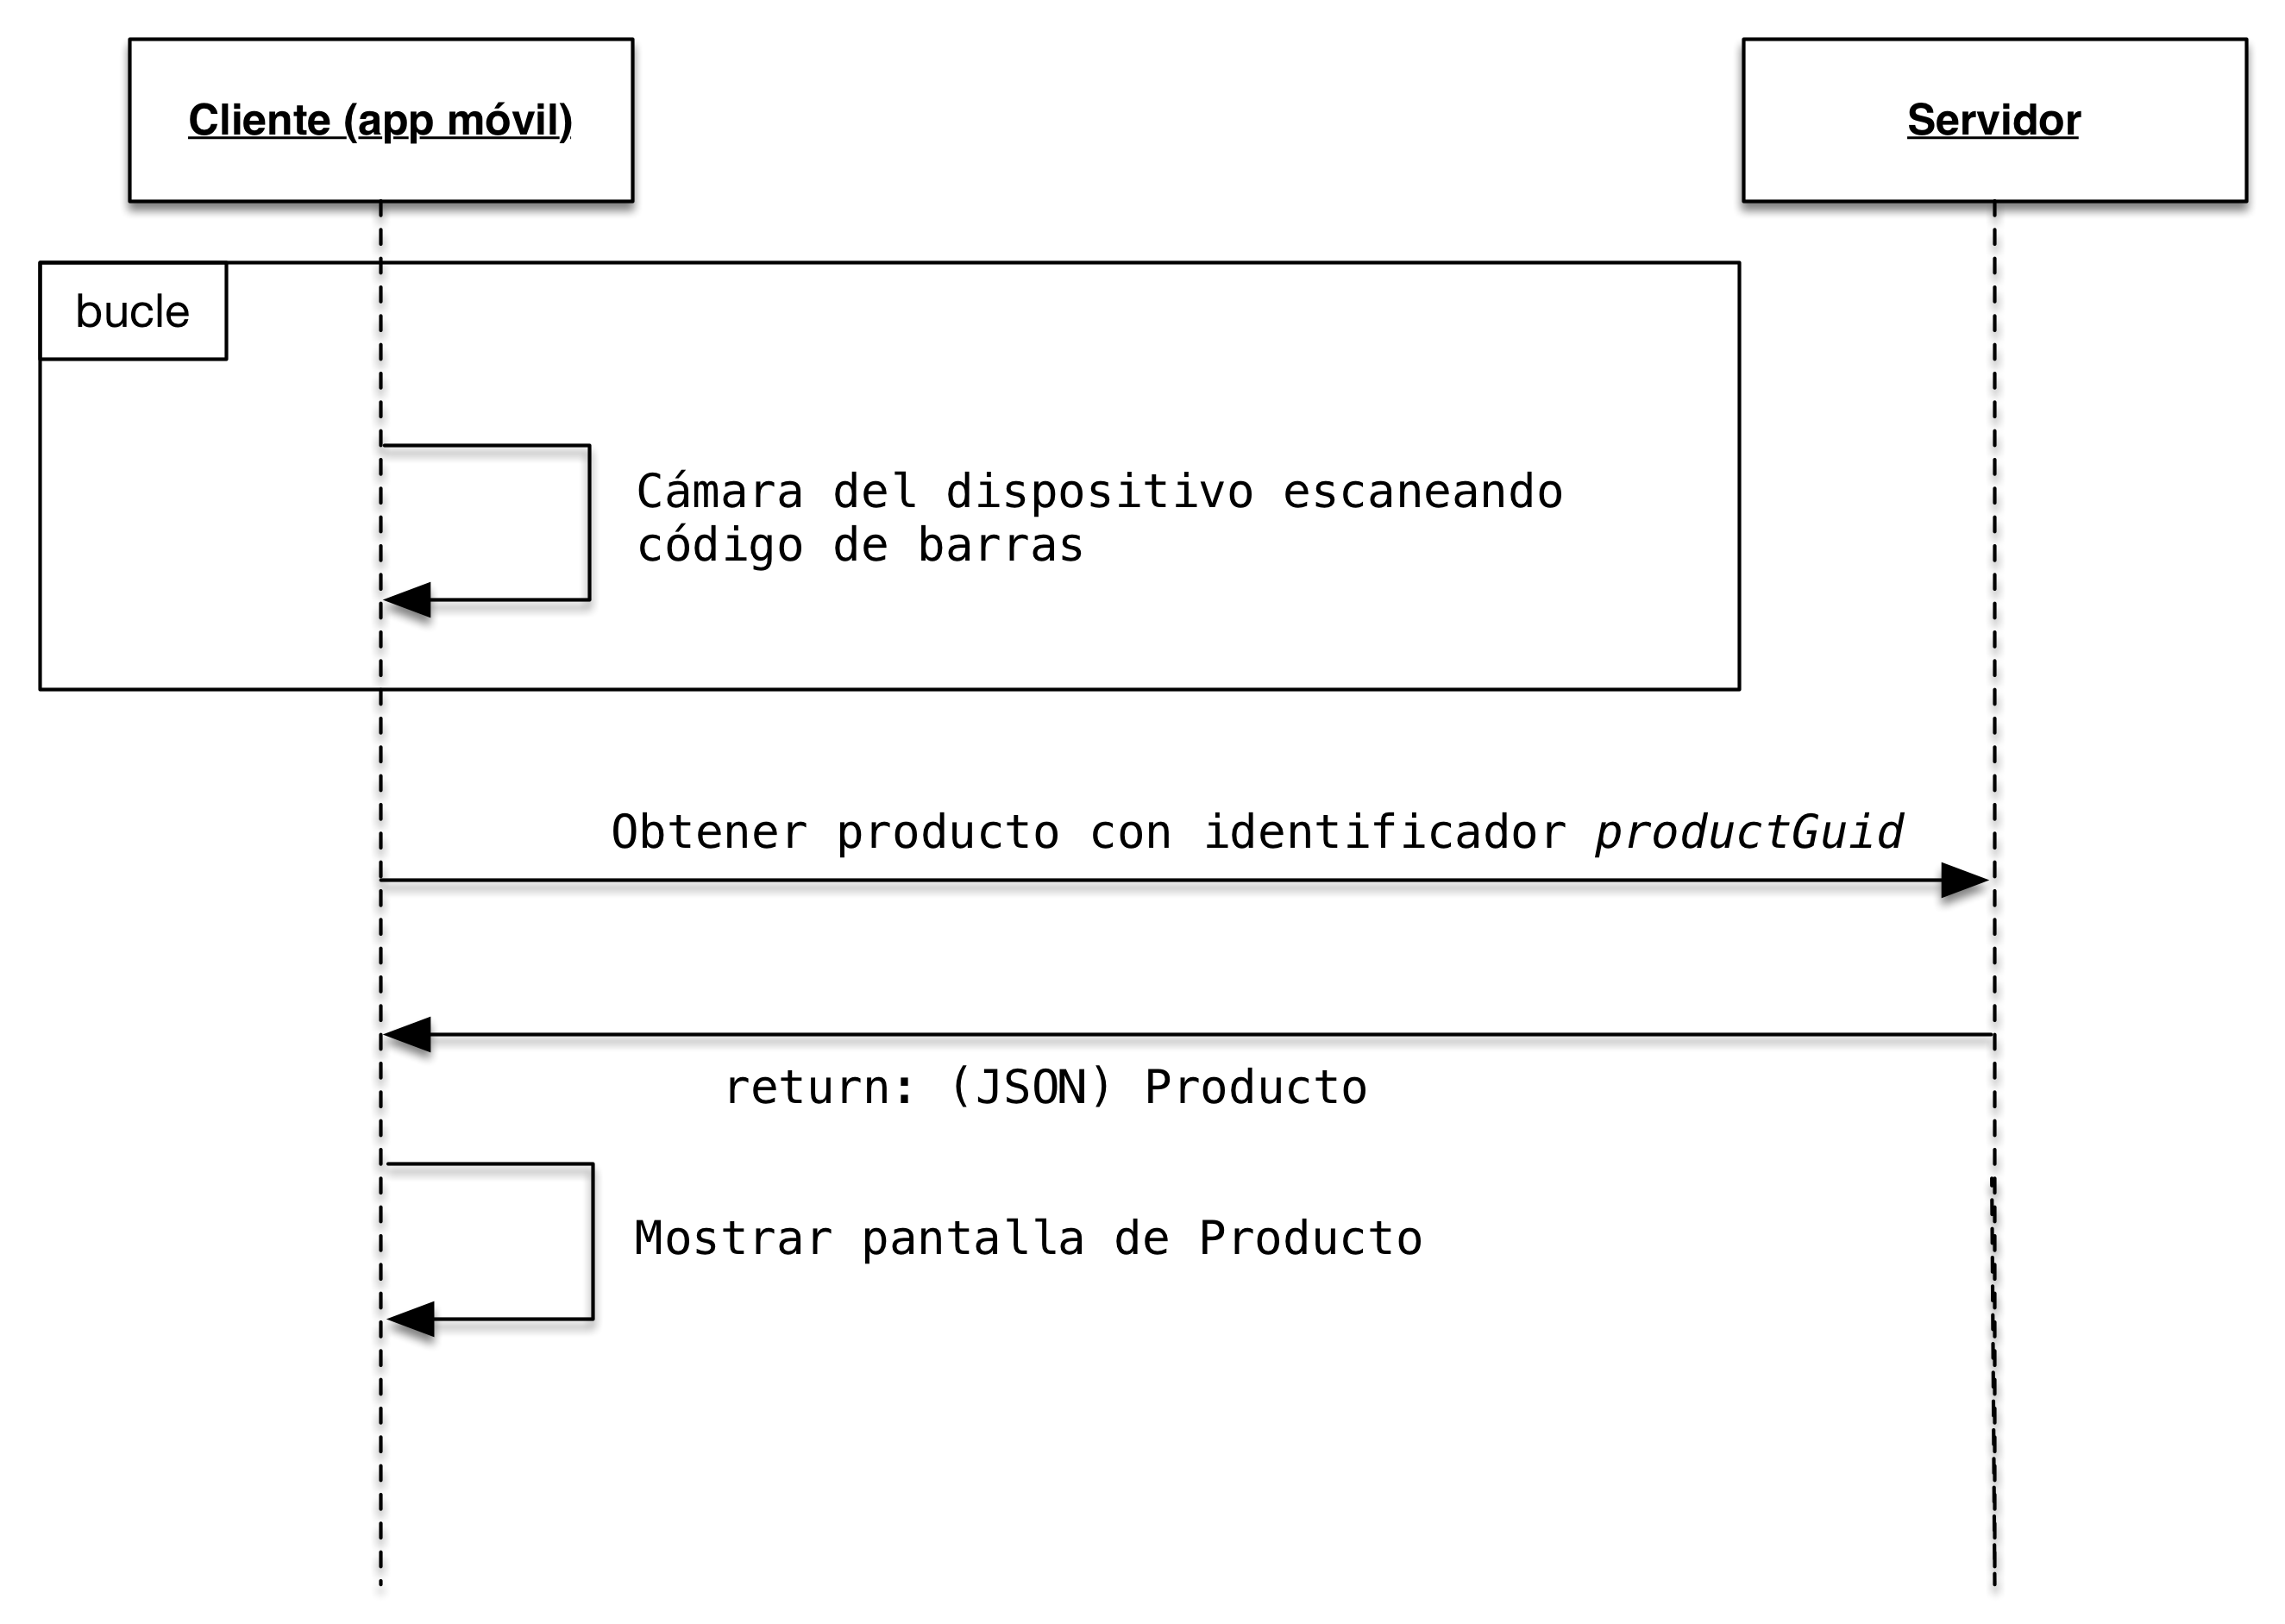
\includegraphics[width=1\textwidth]{./img/diagrama-camara.png}
	\caption{Diagrama de secuencia de lectura de código de barras y búsqueda de producto.}
	\label{fig:diagrama-camara}
\end{figure}

Una vez la aplicación se encuentra en la pantalla descrita en el apartado \ref{sssec:pantalla-info-producto}, el usuario puede pulsar sobre el botón para obtener el stock de ese producto. Tal y como se puede ver en la Figura \ref{fig:diagrama-get-stock}, el cliente obtiene las coordenadas que geolocalizan al dispositivo con una precisión de error mínima (siempre dependiendo de las limitaciones físicas del lugar) y se realiza la llamada al servidor enviando la longitud, latitud y precisión obtenida, junto al identificador de producto.

\begin{figure}[H]
	\centering
		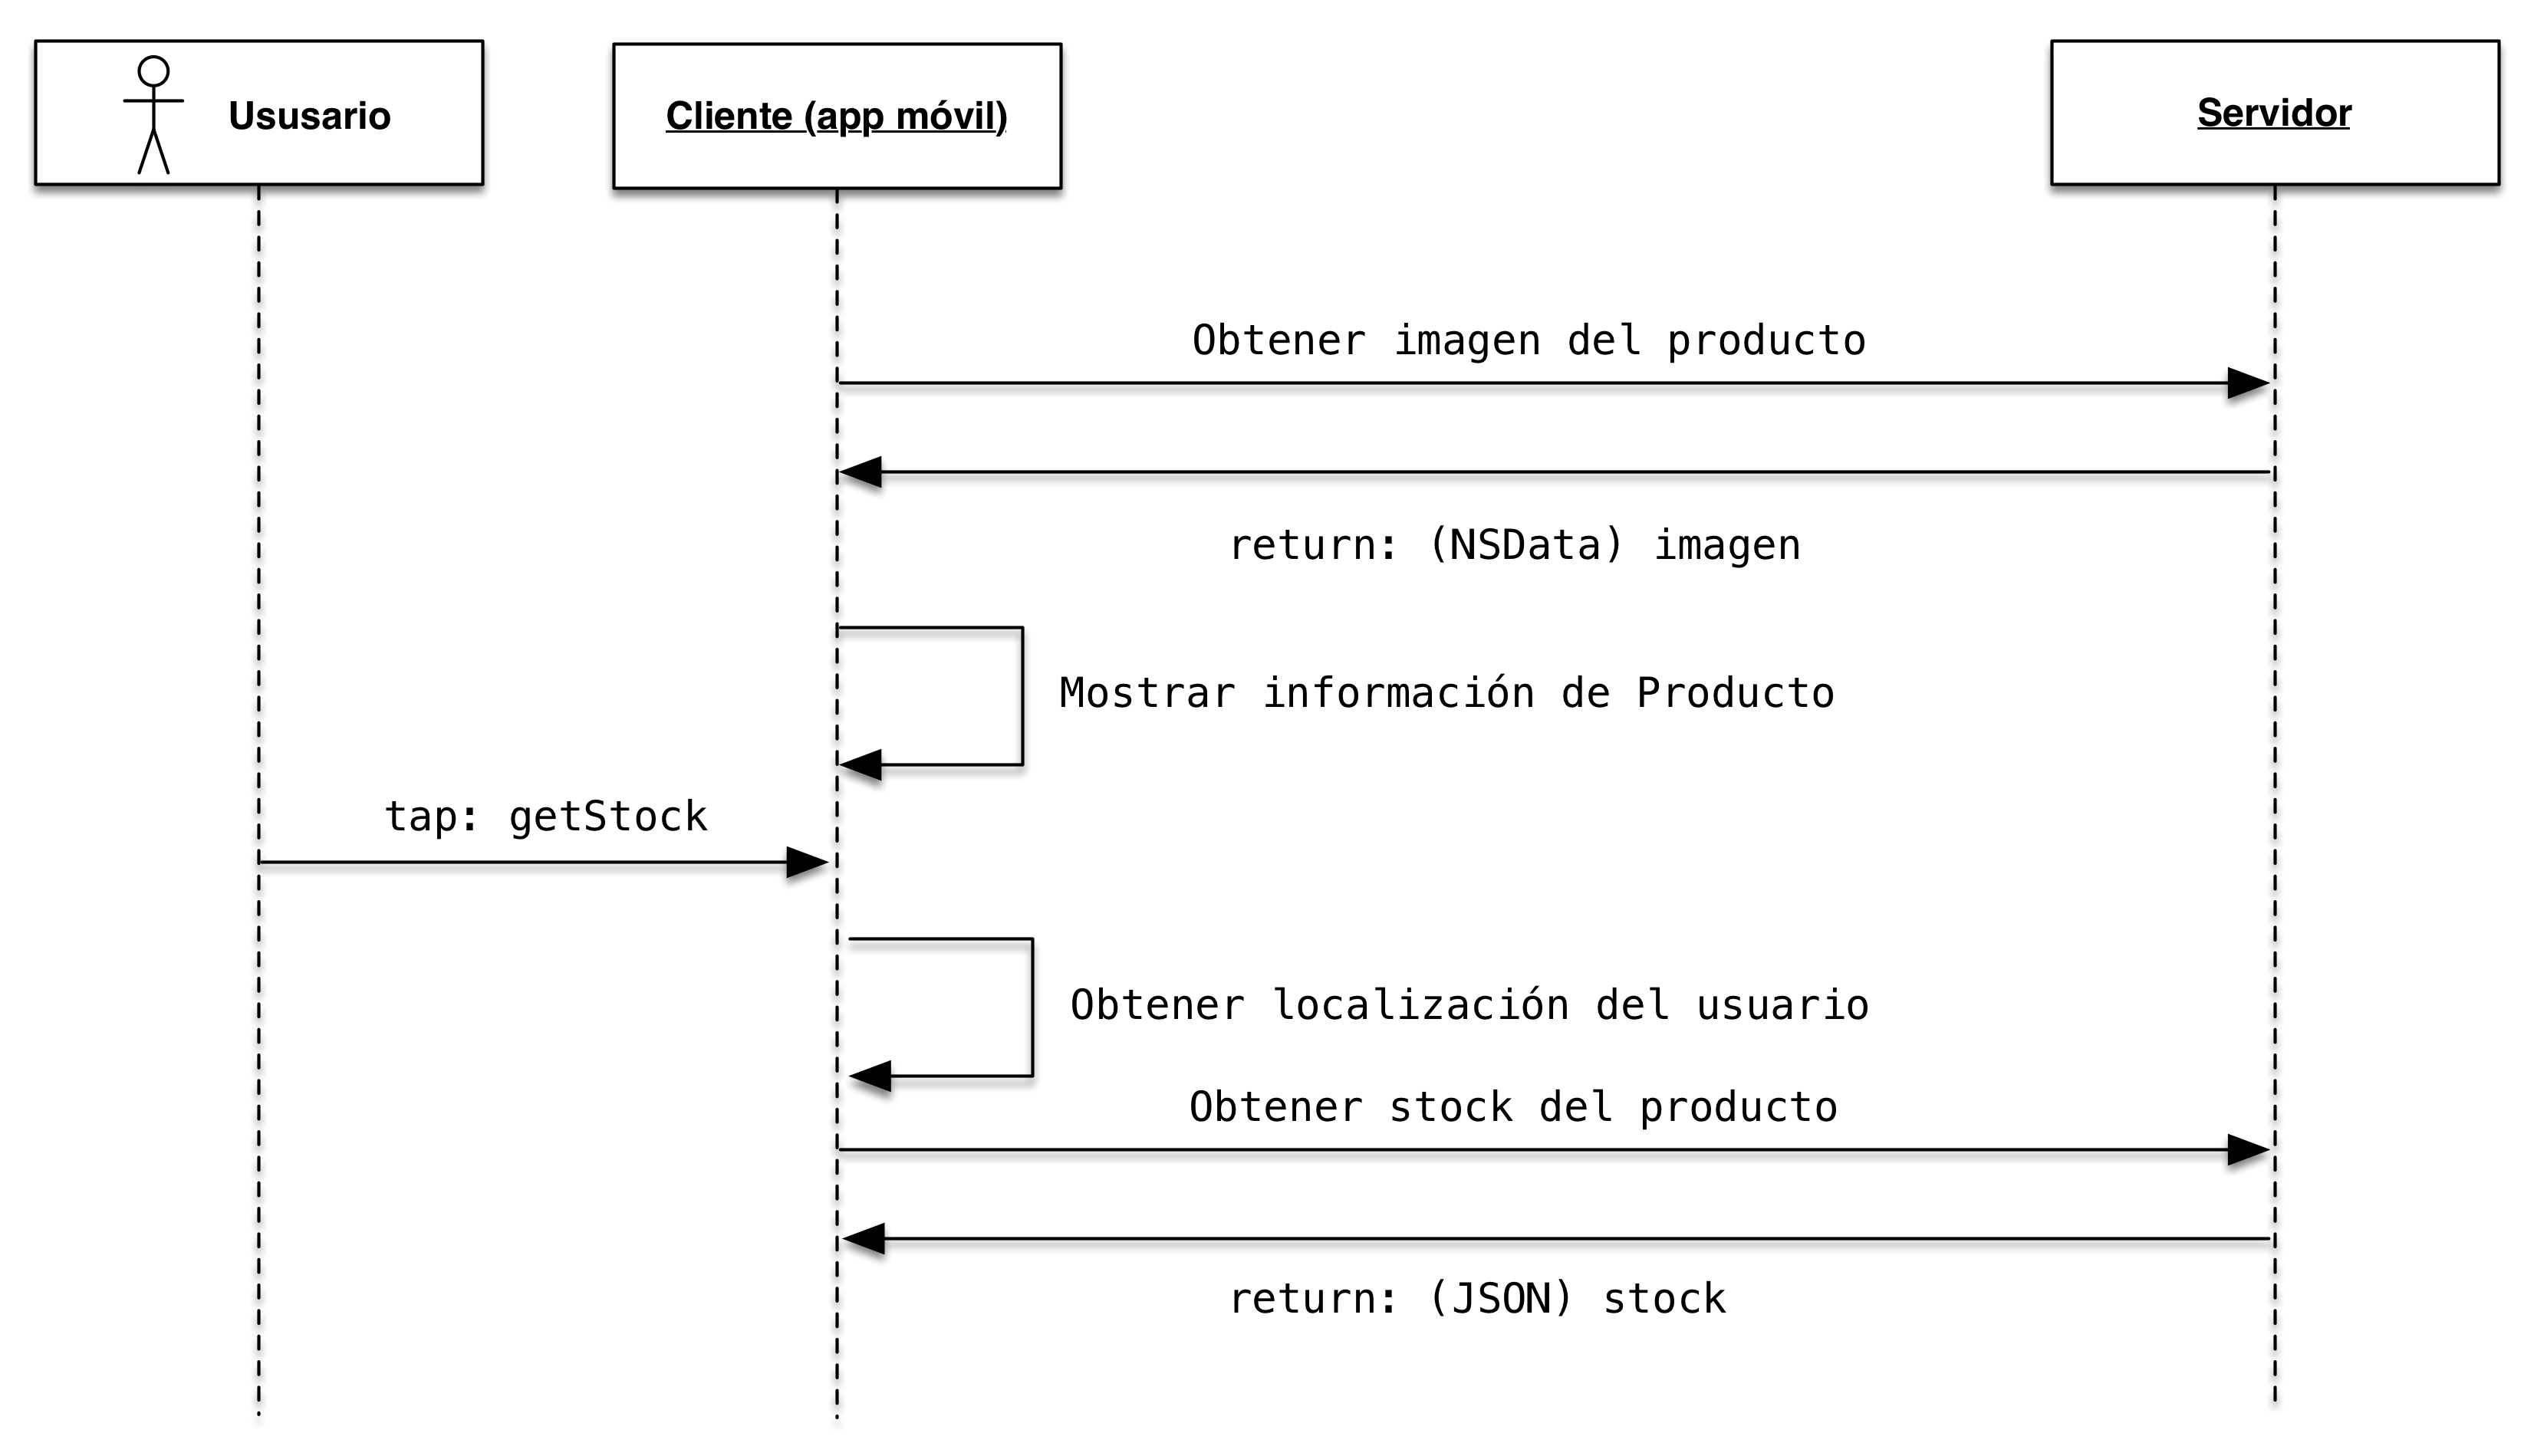
\includegraphics[width=1\textwidth]{./img/diagrama-get-stock.png}
	\caption{Diagrama de secuencia para mostrar el stock de un producto.}
	\label{fig:diagrama-get-stock}
\end{figure}

Cuando el servidor envía los datos de vuelta, el botón usado cambia el texto para mostrar el stock, y sigue estando disponible para realizar nuevamente la acción.

En esta misma pantalla, el usuario también puede pulsar sobre el botón \emph{Tiendas} para obtener un listado con las tiendas y el stock de este producto en cada una.

\begin{figure}[H]
	\centering
		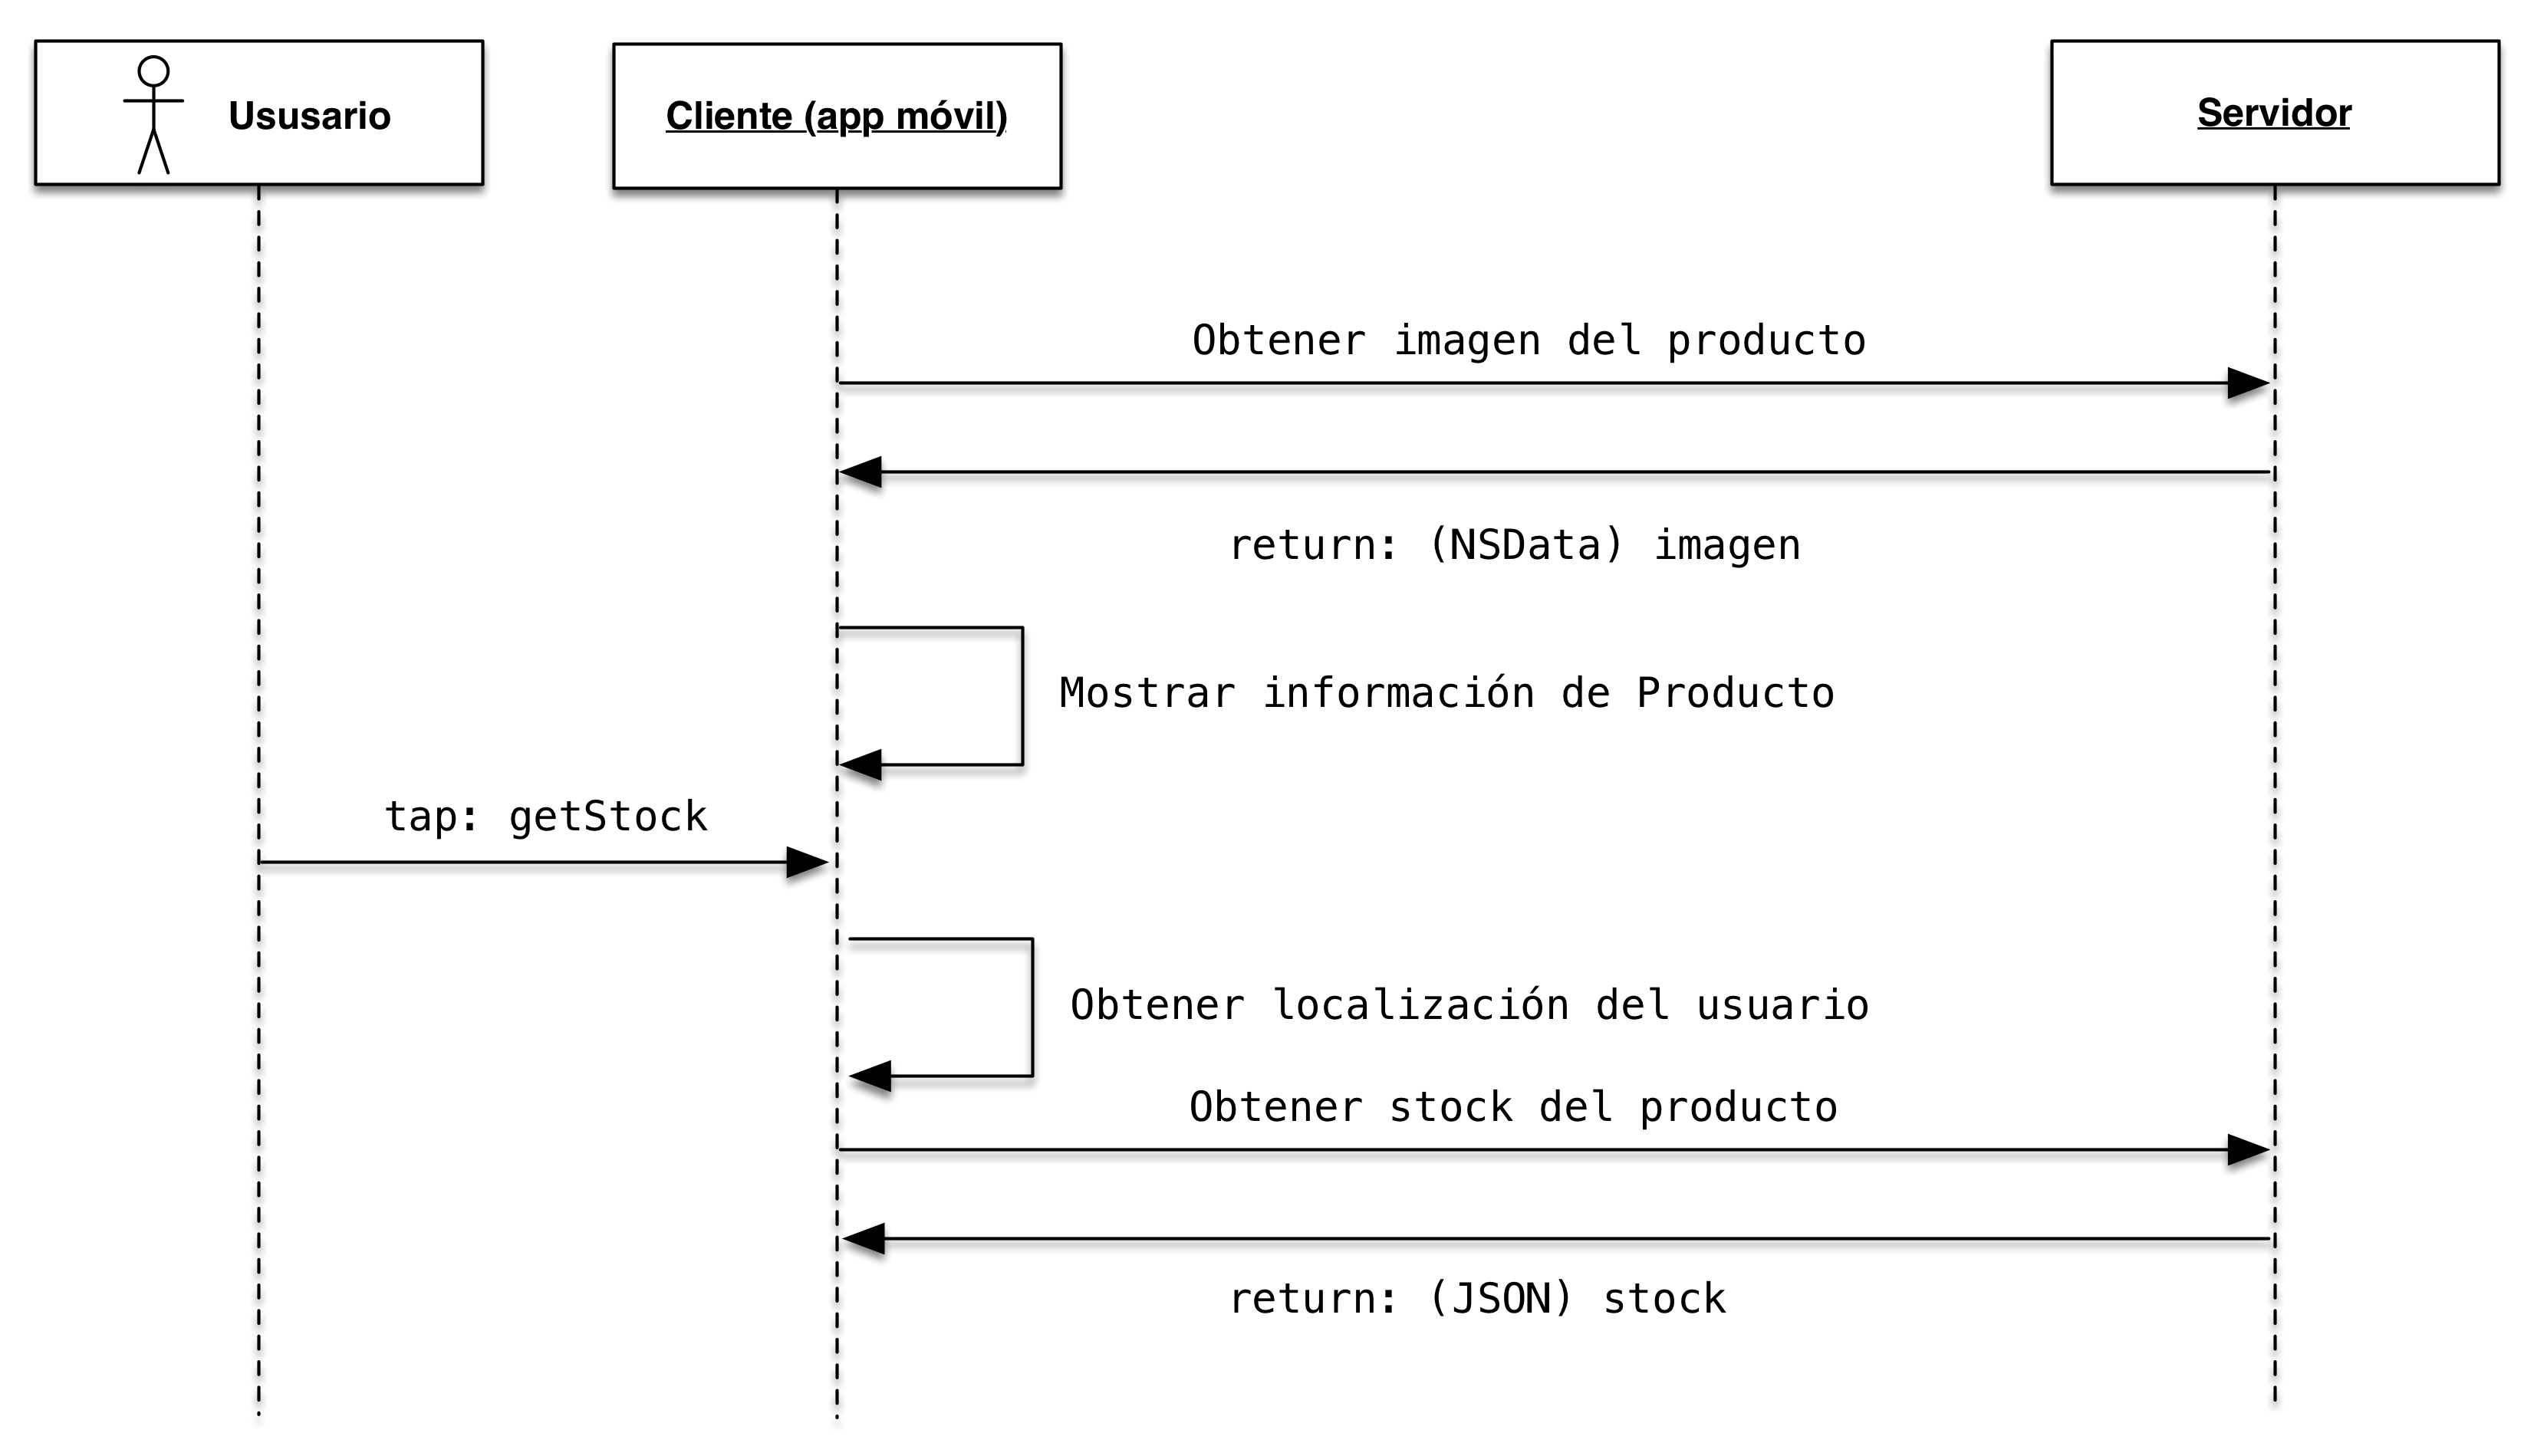
\includegraphics[width=1\textwidth]{./img/diagrama-get-stock.png}
	\caption{Diagrama de secuencia de obtención de listado de tiendas.}
	\label{fig:diagrama-tiendas}
\end{figure}

\section{Servidor}
Este apartado se centra en la parte del servidor. El servidor proporciona por un lado respuestas a las peticiones que le realiza el cliente (devolviendo documentos en lenguaje JSON con los datos) y por otro lado, sigue haciendo las funciones de tienda online.

Como ya se ha comentado antes, la programación del servidor se escapa del ámbito de este PFC, pero es importante conocer la API que se ha creado para este proyecto. A continuación se detallan las llamadas a la API disponibles y el tipo de mensaje que devuelve.

\subsection{/api/v1/Product}
Devuelve un producto en concreto.

Parámetros:
\begin{itemize}
	\item string : productGuid
\end{itemize}

Resultado:
\begin{lstlisting}[language=json]
{
"ProductInfoNodes": [
    {
        "Prod": {
            "ProductGuid": "string",
            "ProductGrp": "string",
            "ProductName": "string",
            "ProductNameTranslate": "string,
            "ListPrice": 0.0,
            "Stock": 0,
            "IsUsedInAnyGroup": true,
            "IsFavorite": true,
            "Properties": {
                "parentGuid": "string",
                "propOwnerTypeGuid": "string",
                "PropDict": {
                    "ALIAS": "string",
                    "_ALIAS": "string",
                    "ATTACHMENT": "string",
                    "_ATTACHMENT": "string",
                    "ATTACHTEXT": "string",
                    "_ATTACHTEXT": "string",
                    "DESCRIPTION": "string",
                    "_DESCRIPTION": "string",
                    "HTMLDESC": "string",
                    "_HTMLDESC": "string",
                    "HYPERLINK": "string",
                    "_HYPERLINK": "string",
                    "LINKTEXT": "string",
                    "_LINKTEXT": "string",
                    "PICTURE1": "string",
                    "_PICTURE1": "string",
                    "PICTURE2": "string",
                    "_PICTURE2": "string",
                    "TEMPLATE": "string",
                    "_TEMPLATE": "string"
                },
                "PropTypeDict": {
                    "ALIAS": "string",
                    "ATTACHMENT": "string",
                    "ATTACHTEXT": "string",
                    "DESCRIPTION": "string",
                    "HTMLDESC": "string",
                    "HYPERLINK": "string",
                    "LINKTEXT": "string",
                    "PICTURE1": "string",
                    "PICTURE2": "string",
                    "TEMPLATE": "string"
                }
            },
            "PropertyGroup": "string",
            "PropCollection": [
                {
                    "PropName": "string",
                    "PropTypeGuid": "string",
                    "PropOwnerRefGuid": "string",
                    "PropGuid": "string",
                    "PropMultilanguage": 0,
                    "PropLangGuid": "string",
                    "PropTransText": "string",
                    "PropValGuid": "string",
                    "PropTransGuid": "string",
                    "SortIndex": 0
                },
                {
                    "PropOwnerRefGuid": "string",
                    "PropGuid": "string",
                    "PropMultilanguage": 0,
                    "PropLangGuid": "string",
                    "PropTransText": "string",
                    "PropName": "string",
                    "PropTypeGuid": "string",
                    "PropValGuid": "string",
                    "PropTransGuid": "string",
                    "SortIndex": 0
                },
                {
                    "PropOwnerRefGuid": "string",
                    "PropGuid": "string",
                    "PropMultilanguage": 0,
                    "PropLangGuid": "string",
                    "PropTransText": "string",
                    "PropName": "string",
                    "PropTypeGuid": "string",
                    "PropValGuid": "string",
                    "PropTransGuid": "string",
                    "SortIndex": 0
                },
                {
                    "PropOwnerRefGuid": "string",
                    "PropGuid": "string",
                    "PropMultilanguage": 0,
                    "PropLangGuid": "string",
                    "PropTransText": "string",
                    "PropName": "string",
                    "PropTypeGuid": "string",
                    "PropValGuid": "string",
                    "PropTransGuid": "string",
                    "SortIndex": 0
                },
                {
                    "PropOwnerRefGuid": "string",
                    "PropGuid": "string",
                    "PropMultilanguage": 0,
                    "PropLangGuid": "string",
                    "PropTransText": "string",
                    "PropName": "string",
                    "PropTypeGuid": "string",
                    "PropValGuid": "string",
                    "PropTransGuid": "string",
                    "SortIndex": 0
                },
                {
                    "PropOwnerRefGuid": "string",
                    "PropGuid": "string",
                    "PropMultilanguage": 0,
                    "PropLangGuid": "string",
                    "PropTransText": "string",
                    "PropName": "string",
                    "PropTypeGuid": "string",
                    "PropValGuid": "string",
                    "PropTransGuid": "string",
                    "SortIndex": 0
                },
                {
                    "PropOwnerRefGuid": "string",
                    "PropGuid": "string",
                    "PropMultilanguage": 0,
                    "PropLangGuid": "string",
                    "PropTransText": "string",
                    "PropName": "string",
                    "PropTypeGuid": "string",
                    "PropValGuid": "string",
                    "PropTransGuid": "string",
                    "SortIndex": 0
                },
                {
                    "PropOwnerRefGuid": "string",
                    "PropGuid": "string",
                    "PropMultilanguage": 0,
                    "PropLangGuid": "string",
                    "PropTransText": "string",
                    "PropName": "string",
                    "PropTypeGuid": "string",
                    "PropValGuid": "string",
                    "PropTransGuid": "string",
                    "SortIndex": 0
                }
            ],
            "propertyIdentifier": "string",
            "IProperties": {
                "parentGuid": "string",
                "propOwnerTypeGuid": "string",
                "PropDict": {
                    "ALIAS": "string",
                    "_ALIAS": "string",
                    "ATTACHMENT": "string",
                    "_ATTACHMENT": "string",
                    "ATTACHTEXT": "string",
                    "_ATTACHTEXT": "string",
                    "DESCRIPTION": "string",
                    "_DESCRIPTION": "string",
                    "HTMLDESC": "string",
                    "_HTMLDESC": "string",
                    "HYPERLINK": "string",
                    "_HYPERLINK": "string",
                    "LINKTEXT": "string",
                    "_LINKTEXT": "string",
                    "PICTURE1": "string",
                    "_PICTURE1": "string",
                    "PICTURE2": "string",
                    "_PICTURE2": "string",
                    "TEMPLATE": "string",
                    "_TEMPLATE": "string"
                },
                "PropTypeDict": {
                    "ALIAS": "string",
                    "ATTACHMENT": "string",
                    "ATTACHTEXT": "string",
                    "DESCRIPTION": "string",
                    "HTMLDESC": "string",
                    "HYPERLINK": "string",
                    "LINKTEXT": "string",
                    "PICTURE1": "string",
                    "PICTURE2": "string",
                    "TEMPLATE": "string"
                }
            },
            "propType": "string"
        },
        "Line": {
            "LineParameter": {
                "AllowLineDisc": true,
                "AllowInvoiceDiscount": true,
                "ItemCustomerDiscountGroup": "string",
                "VATProductPostingGroup": "string",
                "ListPriceIsInclTax": true,
                "Attain_VATBusPostingGrPrice": "string",
                "LineDiscountPct": 0,
                "SubTotal": 0,
                "SubTotalInclTax": 0,
                "OrderLineTotal": 0,
                "InvoiceDiscountAmount": 0,
                "InvoiceDiscountAmountInclTax": 0,
                "ItemCustomerDiscountGroupList": "string"
            },
            "HeaderGuid": "string",
            "CurrencyGuid": "string",
            "LineComment": "string",
            "LineDiscountAmount": 0,
            "LineDiscount": 0,
            "LineGuid": "string",
            "LineNumber": "string",
            "LineTotal": 0,
            "ListPrice": 0.0,
            "ProductGuid": "string",
            "ProductName": "string",
            "Quantity": 0,
            "TaxAmount": 0.0,
            "TotalInclTax": 0.0,
            "VariantCode": "string",
            "IsCalculated": true,
            "VersionGuid": "string",
            "ListPriceInclTax": 0.0,
            "LineDiscountAmountInclTax": 0,
            "VariantName": "string",
            "TaxPct": "string"
        },
        "VariantDict": "string",
        "Messages": "string",
        "ProductRelations": "string"
    }
],
"TotalCountInDb": 0,
"Header": {
    "Lines": [
        {
            "LineParameter": {
                "AllowLineDisc": true,
                "AllowInvoiceDiscount": true,
                "ItemCustomerDiscountGroup": "string",
                "VATProductPostingGroup": "string",
                "ListPriceIsInclTax": true,
                "Attain_VATBusPostingGrPrice": "string",
                "LineDiscountPct": 0,
                "SubTotal": 0.0,
                "SubTotalInclTax": 0.0,
                "OrderLineTotal": 0,
                "InvoiceDiscountAmount": 0,
                "InvoiceDiscountAmountInclTax": 0,
                "ItemCustomerDiscountGroupList": "string"
            },
            "HeaderGuid": "string",
            "CurrencyGuid": "string",
            "LineComment": "string",
            "LineDiscountAmount": 0,
            "LineDiscount": 0,
            "LineGuid": "string",
            "LineNumber": "string",
            "LineTotal": 0.0,
            "ListPrice": 0.0,
            "ProductGuid": "string",
            "ProductName": "string",
            "Quantity": 0,
            "TaxAmount": 0.0,
            "TotalInclTax": 0.0,
            "VariantCode": "string",
            "IsCalculated": true,
            "VersionGuid": "string",
            "ListPriceInclTax": 0.0,
            "LineDiscountAmountInclTax": 0,
            "VariantName": "string",
            "TaxPct": "string"
        }
    ],
    "HeaderParameter": {
        "AllowLineDisc": true,
        "CustomerGuid": "string",
        "CustomerDiscountGroup": "string",
        "PriceGroupCode": "string",
        "InvoiceDiscountCode": "string",
        "VATBusinessPostingGroup": "string",
        "CurrencyGuid": "string",
        "SubTotal_InvoiceDiscount": 0.0,
        "SubTotal_ServiceCharge": 0.0
    },
    "CreatedDate": "string",
    "CurrencyGuid": "string",
    "CustomerPONumber": "string",
    "HeaderComment": "string",
    "HeaderGuid": "string",
    "InvoiceDiscount": 0,
    "ModifiedDate": "string",
    "MultiCartDescription": "string",
    "MultiCartStatus": "string",
    "ServiceCharge": 0,
    "SubTotal": 0.0,
    "TaxAmount": 0.0,
    "TaxCode": "string",
    "TotalInclTax": 0.0,
    "UserGuid": "string",
    "Total": 0.0,
    "CustomerReference": "string",
    "ShippingHandlingProviderGuid": "string",
    "IsCalculated": true,
    "VersionGuid": "string",
    "SubTotalInclTax": 0.0,
    "ServiceChargeInclTax": 0,
    "InvoiceDiscountInclTax": 0,
    "ShippingAmount": 0,
    "ShippingAmountInclTax": 0,
    "HandlingAmount": 0,
    "HandlingAmountInclTax": 0,
    "PaymentStatus": "string",
    "PaymentError": "string",
    "ShipToAddress1": "string",
    "ShipToAddress2": "string",
    "ShipToCityName": "string",
    "ShipToCompanyName": "string",
    "ShipToContactName": "string",
    "ShipToCountryGuid": "string",
    "ShipToCountryName": "string",
    "ShipToCountyName": "string",
    "ShipToEmailAddress": "string",
    "ShipToStateName": "string",
    "ShipToZipCode": "string",
    "ShipToShippingAddressGuid": "string",
    "Address1": "string",
    "Address2": "string",
    "CityName": "string",
    "CompanyName": "string",
    "ContactName": "string",
    "CountryGuid": "string",
    "CountryName": "string",
    "CountyName": "string",
    "EmailAddress": "string",
    "StateName": "string",
    "ZipCode": "string",
    "ShippingAddressGuid": "string",
    "PaymentMethod": "string",
    "InvoiceDiscountPct": "string",
    "TaxPct": "string",
    "PricesIncludingVat": true,
    "VatTypes": "string"
}
\end{lstlisting}

\subsection{/api/v1/GetAllLocationsForProduct}
Devuelve un listado con el stock del producto en cuestión en cada tienda.

Parámetros:
\begin{itemize}
	\item string : productGuid
\end{itemize}

Resultado:
\begin{lstlisting}
	
\end{lstlisting}

\subsection{/api/v1/GetStockInLocation}
Devuelve el stock de un producto en una tienda dada la localización en coordenadas.

Parámetros:
\begin{itemize}
	\item string : productGuid
	\item double : latitude
	\item double : longitude
	\item double : accuracy
\end{itemize}

Resultado:
\begin{lstlisting}
	
\end{lstlisting}
\chapterend